\chapter{Simulation in CUORE}
\label{ch:Simulation in CUORE}

In CUORE, simulation plays a large role in characterizing both signal and background events in the detectors.
As noted in \autoref{eq:sensitivity_short}, any search for \zeronubb~needs to be able to fully understand the background contribution in the region of interest.
This is certainly a non-trivial problem, however, as there are radioactive contaminants in varying levels all throughout the cryostat, and the data measured in CUORE is a function of all of them simultaneously.
Because of the lack of an signal ``off" mode in CUORE\footnote{Which could be achieved by having $^{130}$Te-depleted crystals, for example.}, these backgrounds cannot be subtracted from a signal, and require a careful understand of them to properly identify the physics of interest in CUORE.
One of the main sources of understanding we have for these backgrounds comes from simulations of each source, allowing them to be studied in isolation or in groups to better understand their effects on the data.
\section{Monte Carlo Method Overview}
The general method by which all simulation is run is called the Monte Carlo method.
The idea behind this method is a simple one: for many problems that have a computationally intractable solution, a simpler problem is to repeatedly and randomly sample possible cases to solve.

For example, calculating $\pi$ can be done via a simple Monte Carlo method by sampling random points in a unit square and dividing the number of points that are inside an inscribed circle by the total number of points.
When the sample size is large, this method works well to determine the value of $\pi$.
As noted above, in CUORE we are generally interested in determining what the distribution of timing, energy, and location of particular types of events is, and thus we apply these Monte Carlo methods to determine the effect by sampling produced particles and their interactions in the cryostat.
We also use other types of Monte Carlo, which are discussed more in \autoref{sec:MCMC}.

An example in the case of CUORE comes from the fact that determining the entire energy spectrum coming from the decays in a $^{60}\textrm{Co}$ contamination on a copper frames is a difficult problem to solve analytically, but it is more straightforward to solve for the propagation and energy deposition of individual particles emitted from the copper frames.
Furthermore, these types of problems are highly parallelizable and benefit strongly from large computing clusters.

\section{Geant4 Simulation Toolkit}
The Geant4 toolkit is a software widely used in the physics community to solve these sorts of physics problems where particles pass through matter using Monte Carlo methods \cite{AGOSTINELLI2003250, 528223, ALLISON2016186}.
Using this toolkit, one can define the detector geometry and materials and then propagate particular particles with varying physics models.
This software uses a similar procedure as described above to simulate the effects from radioactive decays in the cryostat.
First, a primary particle is generated in a particular material, e.g. a decay in the $^{232}$Th decay chain in the copper frames, and that particle is then propagated throughout the cryostat in a series of steps.
At each step, one of the possible physics processes is sampled probabilistically and the energy lost due to interactions or creation of daughter particles is taken into account and particle (primary and any daughters) are transported along another step until their energies are lower than a defined threshold.
Geant4 uses ``physics lists" to determine the physics that is sampled from for the interactions at each step, and CUORE utilizes the \textit{Livermore} and \textit{Shielding} physics lists to account for the low-energy electromagnetic interactions down to 250 eV and for higher-energy neutron penetration, respectively.
In a detector, the energy lost by the particle and its daughters during steps inside the volume can then be recorded as the energy deposited in the detector and corresponds to what is measured by the NTDs in CUORE.
However, the only information that is recorded here is the energy deposited in each crystal by each particle and the timing information\footnote{For decays generated through a decay chain, if there is $>1$ year between events, the next generated particles in the chain are moved to a separate location in the generating volume.}

\section{CUORE Reconstruction in Geant4}
CUORE utilizes Geant4\footnote{Version 9.6.p03} and has recreated the entire cryostat in its own software package, called \textit{qshields}, shown in \autoref{fig:CUORE_cyrostat_MC} and \autoref{fig:CUORE_crystals_MC}.
For the reconstruction, there is a balancing act in the reconstruction between the full fidelity of the recreation and the need for simplicity and reducing the load on CPU resources.
For example, there are 4 thermalizing blocks for the calibration system on the 4-K stage, see \autoref{fig:4K_thermalizer_schematic}, but they are not included in the reconstruction of the cryostat.
However, the detectors and their nearest components in the detector region do require as high-fidelity of a reconstruction as possible, as their particular geometry plays a significantly larger role in the simulated physics\footnote{For example, consider an $\alpha$ emitted from the external lead versus one from the copper frames around the detectors.
While it is certainly important to each what the geometry looks like, the $\alpha$ from the external lead will never make it to the detectors.}.
This can be seen in \autoref{fig:CUORE_crystals_MC}.
In addition, in order to reduce the computation time for propagating these particles, in the internal and external lead shielding, particles are propagated to a minimum of a step size of 1 cm as they are less likely to interact with the detectors, while the other components have a minimum step size of 0.1 cm.

\begin{figure}[htbp]
    \centering
    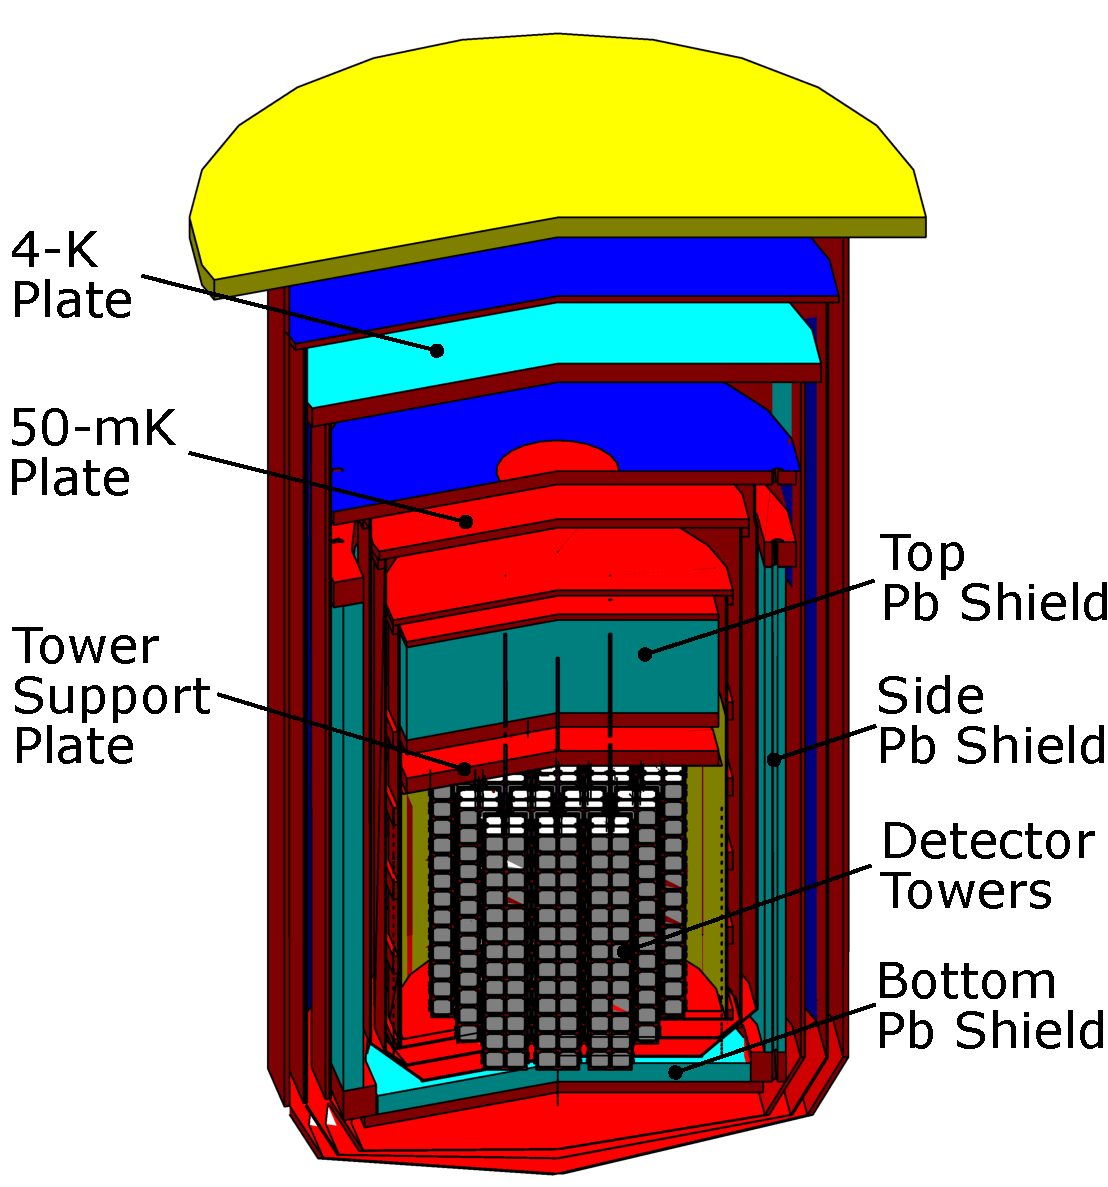
\includegraphics[height=0.6\paperheight]{Figures/CUORE_cryostat_labelled.pdf}
    \caption[A rendering of the CUORE crysotat as it is reconstructed in Geant4]
    {A rendering of the CUORE cryostat as it is reconstructed in Geant4.
    The shielding is cut away show the inside of the cryostat and some of the tubes for the internal Detector Calibration System.
    Compare this rendering with the CAD rendering in \autoref{fig:cryostat_cad_cutout}.}
    \label{fig:CUORE_cyrostat_MC}
\end{figure}

\begin{figure}[htbp]
    \centering
    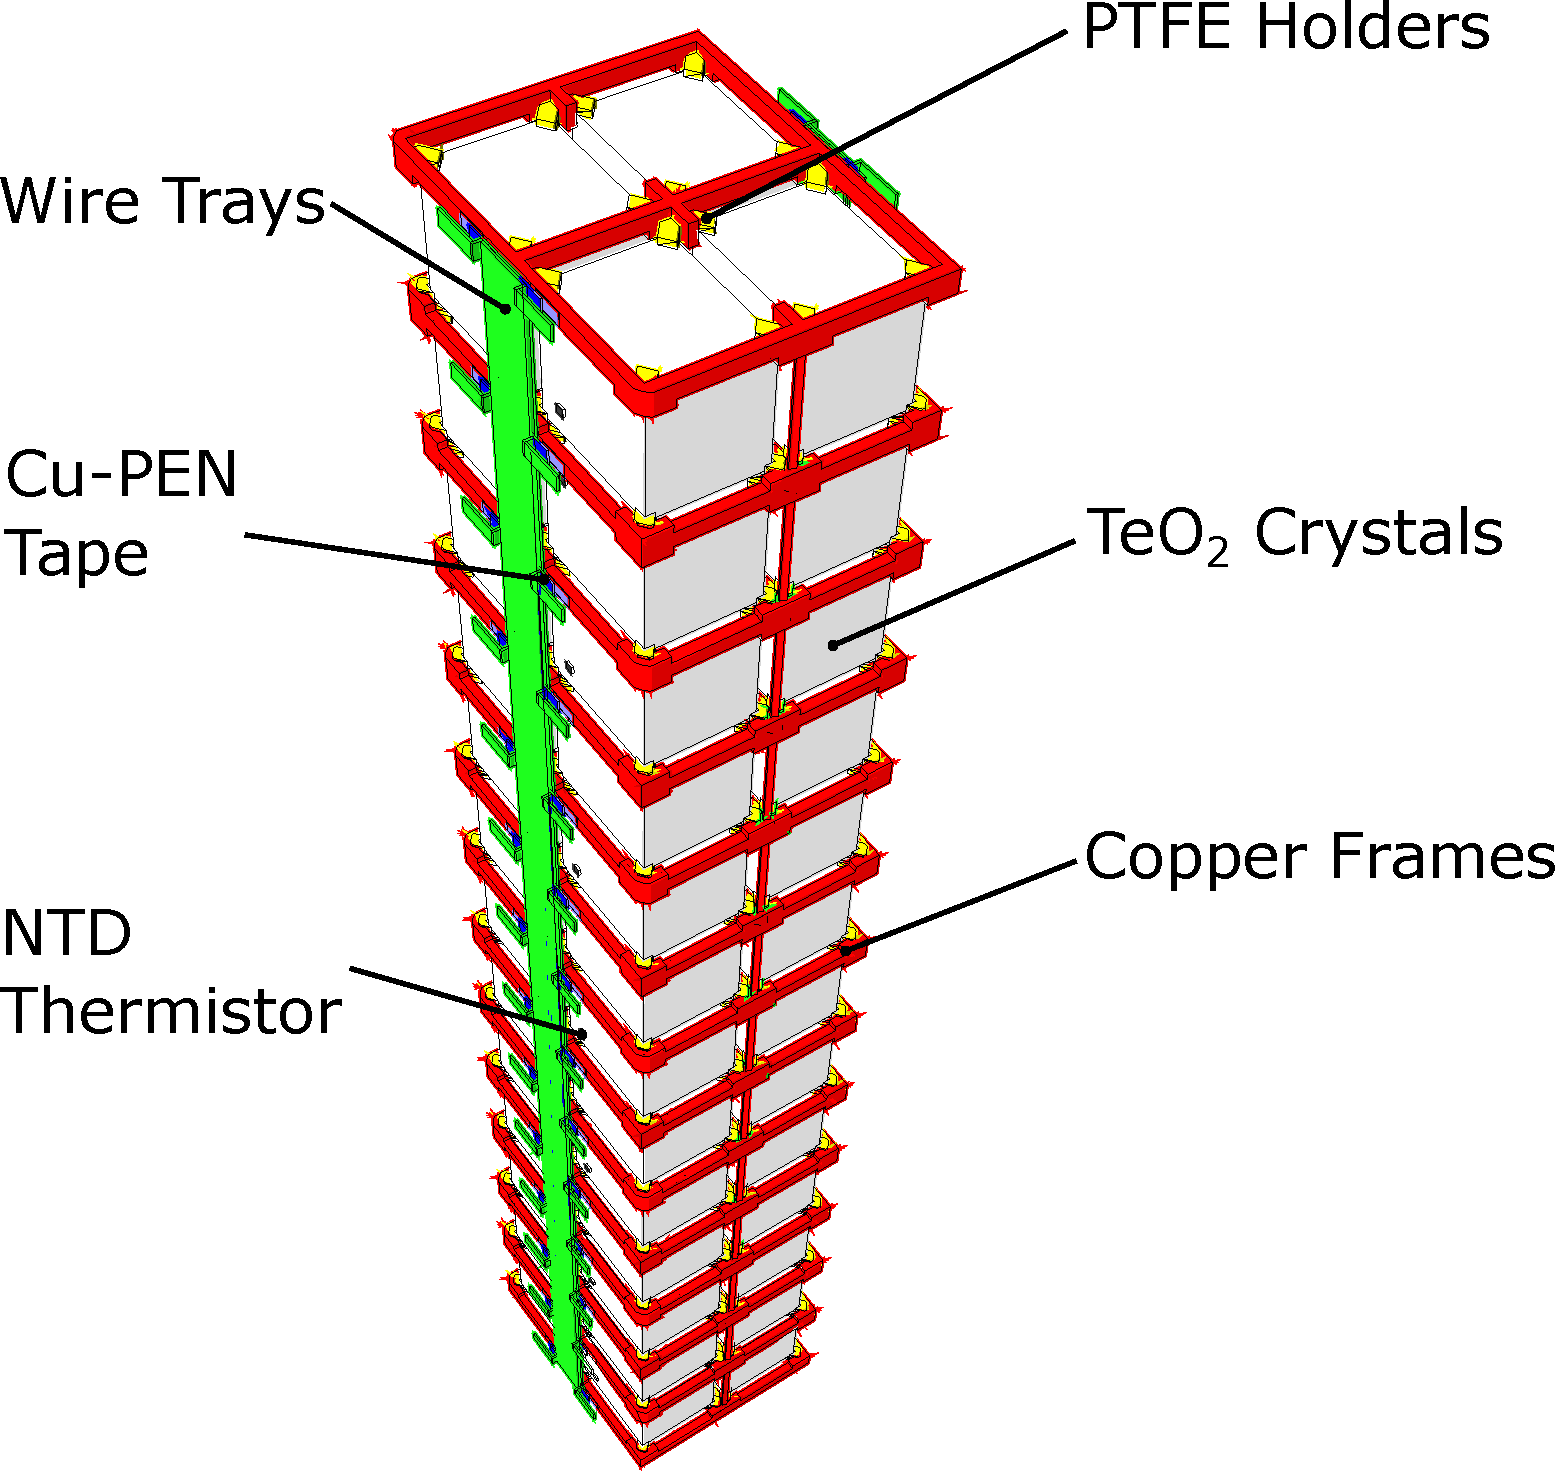
\includegraphics[height=0.3\paperheight]{Figures/Crystals_rotated_labelled.pdf}
    \caption[A visualization of the CUORE crystals as they are reconstructed in Geant4]
    {A visualization of the CUORE crystals as they are reconstructed in Geant4.
    Care is taken to precisely replicate these components in close proximity to the crystals.
    The Si heaters, however, are not recreated due to their small size relative to the minimum step size.}
    \label{fig:CUORE_crystals_MC}
\end{figure}

\section{Simulating Detector Response}
The physics simulation in Geant4 is only one part of the two-step process in performing physics simulations in CUORE.
Geant4 does not take into consideration the actual detector response to the physics, such as pileup between the physics simulated in parallel.
To then be able to characterize this detector response, another software package called \textit{g4cuore} is used.
This software works to replicate the software steps described in \autoref{ch:Data Acquisition and Processing} to turn the raw output of Geant4 and \textit{qshields} into a processed spectrum similar to what would be observed in the data.
In particular, the detector effects that are applied are:
\begin{itemize}
    \item event rates
    \item detector resolution
    \item pileup rejection and detector dead time
    \item energy thresholds
    \item coincidences 
    \item quenching factors
\end{itemize}
In addition, not only does applying these effects allow for simulating the detector response, it also allows this detector response to be studied.
For example, by varying the event rate, the effect of a particular pileup rejection cut can be studied as shown in \autoref{fig:pileup_effects}.
Similarly, by varying the coincidence window and the event rate, the relative rates of real and accidental coincidences can be studied as well.


\section{Simulation Benchmarking}

As simulations are performed on multiple clusters and as updates are made to the software, it is important to perform benchmarking to discover bugs and other errors in the simulation.
In addition, benchmarking is useful when creating tagged versions of software as each tagged version can be checked back against earlier versions.
To benchmark, a representative sample of simulations is produced by qshields and compared to the spectra produced by an earlier version of qshields.
In this way, unexpected issues can be discovered and the effects of changes to the simulation can be observed.
For example, errors were discovered in the way that the copper frames and PTFE holders were implemented in \textit{qshields} and this effect was quantified by performing this benchmarking of the simulations, as shown in \autoref{fig:PTFESx_M1}.
In general, observing a difference in the spectral shape is evidence of an issue with the physics, such as a missing Geant4 patch, while observing a difference in the number of observed counts is generally caused by geometry.

\begin{figure}
    \centering
    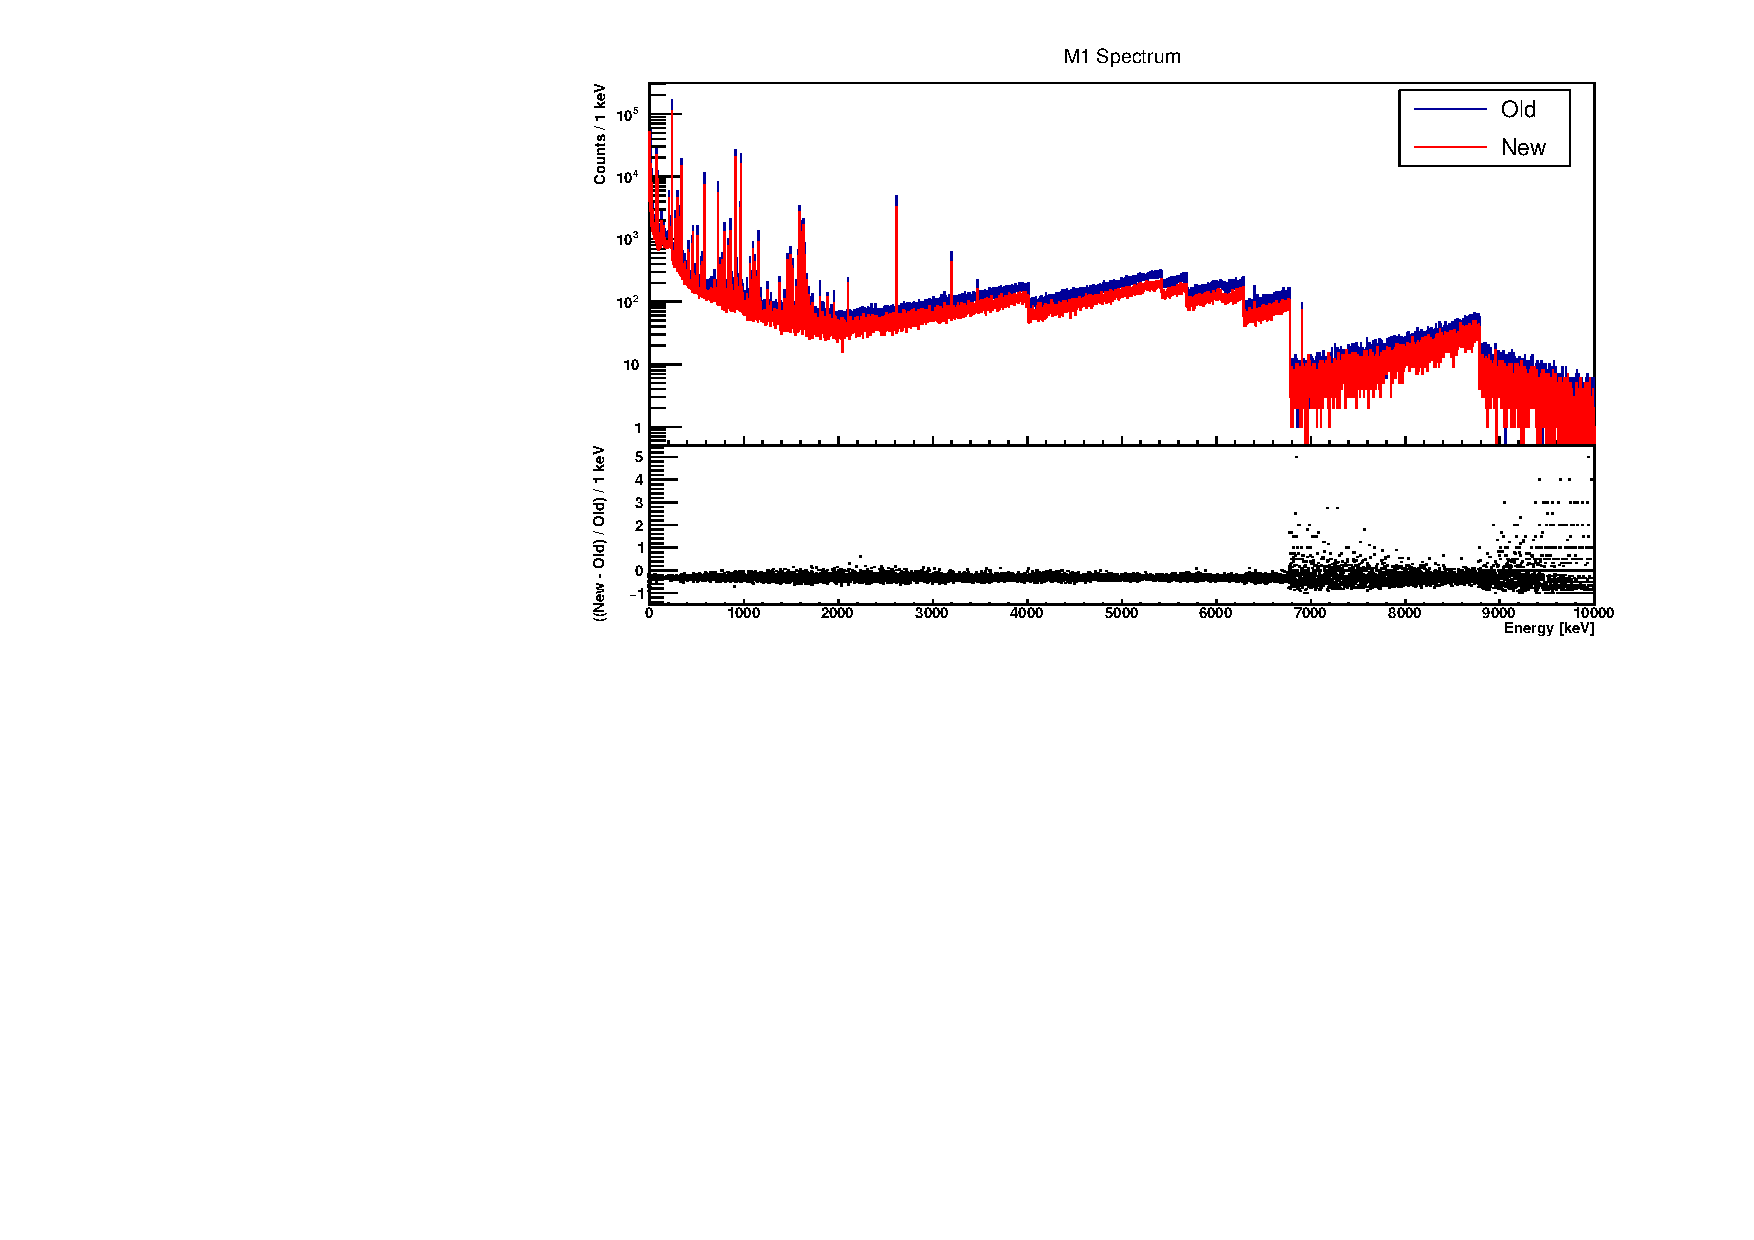
\includegraphics[width=0.8\linewidth]{Figures/PTFESx_M1.pdf}
    \caption[The changes in the simulated spectra due to fixes in the geometry in \textit{qshields}]
    {The changes in the simulated spectra due to fixes in the geometry in \textit{qshields}.
    With the same number of decays generated, a roughly 20\% drop in the number of events is observed while preserving the spectral shape.}
    \label{fig:PTFESx_M1}
\end{figure}